\documentclass[a4paper,oneside,12pt]{amsart}

%\usepackage[spanish, activeacute]{babel}
\usepackage[utf8]{inputenc}
%\usepackage[latin1]{inputenc}
\usepackage{latexsym}
\usepackage{multicol}
\usepackage{enumerate}
\usepackage{enumitem}
\usepackage[heightrounded]{geometry}
\geometry{top=2cm,bottom=2cm,left=2cm,right=2cm}
\usepackage{graphicx}
\usepackage{tikz}
\usepackage{amssymb}
\usepackage{tikz-network}

\DeclareMathOperator{\cond}{cond}
\DeclareMathOperator{\Id}{Id}
\DeclareMathOperator{\re}{Re}
%\DeclareMathOperator{\im}{Im}
\newcommand{\I}{\mathbb{I}}
\newcommand{\R}{\mathbb{R}}
\newcommand{\Q}{\mathbb{Q}}
\newcommand{\C}{\mathbb{C}}
\newcommand{\Z}{\mathbb{Z}}
\newcommand{\N}{\mathbb{N}}
\DeclareMathOperator{\im}{Im}

\newcommand{\nombremateria}
{Investigaci\'on Operativa}
\newcommand{\nombrecuatrimestre}
    {Segundo cuatrimestre de 2021}
\newcommand{\numeroparcial}
    { Tercer Parcial }
\newcommand{\fecha}
    {28 de Octubre de 2022}
\newcommand{\numerotema}
    {\bf 1}

%\oddsidemargin -1cm \evensidemargin -1cm \textwidth 17.5cm
%topmargin 1.2cm \textheight 25cm
%\setlength{\textheight}{25cm}

\def \ds{\displaystyle}
\theoremstyle{definition}
\newtheorem{quest}{Ejercicio}
\thispagestyle{empty}

\begin{document}

\hfill \hfill
\begin{tabular}[c]{|c|c|c|c|c|}
\hline 
1 & 2 & 3 & 4 & Calificaci\'on \\ \hline \hline
\hspace{1.2 cm} & \hspace{1.2 cm} & \hspace{1.2 cm} & \hspace{1.2 cm}  &\hspace{1.5 cm} \\
\hspace{1.2 cm} & \hspace{1.2 cm} & \hspace{1.2 cm} & \hspace{1.2 cm}  &\hspace{1.5 cm} \\ \hline

\end{tabular}

\vspace{-1cm}

\noindent Nombre y apellido:

\vspace{0.2cm}

\noindent Número de libreta:

\noindent \hrulefill 

\smallskip
\renewcommand{\baselinestretch}{1.1}

\begin{center}
	\large \textbf{\nombremateria} 
	
	\numeroparcial -- \fecha
\end{center}

\noindent\textit{Para aprobar el parcial deberá obtenerse un puntaje mayor o igual que 4. \textbf{Entregue todos los ejercicios en hojas separadas.}}

\vspace{.6cm}
\renewcommand{\theenumi}{\textbf{\arabic{enumi}}}

%%% EMPIEZA EL EJERCICIO 1 %%%

\begin{quest}\verb|[3 pts.]|  
Demostrar las siguientes afirmaciones para un grafo $G$. Cada ítem se puede demostrar individualmente, no es necesario utilizar el resultado de los demás.
\begin{enumerate}[label=\alph*)]
    \item \verb|[0.5 pts.]| Si $\delta(G)\geq k$ ($k\in\mathbb{N}$), entonces $G$ tiene un camino simple de largo $k$. (Recordar que la longitud de un camino está dada por su cantidad de aristas).
    % \item Sea $G=(V_1\cup V_2, E)$ un grafo bipartito Hamiltoniano, entonces $|V_1|=|V_2|$.
    \item \verb|[1.5 pts.]| Si $G$ tiene $n$ vértices ($n\geq 3$) y $\frac{1}{2}(n-1)(n-2)+2$ aristas, entonces $G$ tiene un ciclo Hamiltoniano. \textbf{Sugerencia:} utilizar el teorema de Ore.
    \item  \verb|[1 pt.]| Sea $G$ un grafo conexo pesado. Sea $e$ la arista de mayor peso de un ciclo de $G$ (es decir $w(e)>w(e')$ para toda arista $e'\neq e$ del ciclo). Probar que $e$ no pertenece a ningún árbol generador mínimo de $G$.
\end{enumerate}

\end{quest}

%%% TERMINA EL EJERCICIO 1 %%%

%%% EMPIEZA EL EJERCICIO 3 %%%


\begin{quest}\verb|[2.5 pts.]| 
A un curso de posgrado asisten alumnes de distintas disciplinas. El trabajo final será en grupos y a cada uno de ellos le será asignado un tema distinto. Para alentar la interdisciplinariedad, la profesora propone que se formen grupos de manera tal que cada estudiante no comparta campo de investigación con sus compañeres de equipo. Los datos sobre les estudiantes y sus campos de investigación son los siguientes:
\begin{table}[htpb!]
    \centering
    \begin{tabular}{|c|l|}\hline
        Estudiante & Campo(s) de investigación  \\\hline
        $1$ & Matemática \\
        $2$ & Matemática, Ciencia de Datos \\
        $3$ & Matemática, Computación, Ciencia de Datos \\
        $4$ & Computación, Biología \\
        $5$ & Computación, Ciencia de Datos\\\hline
    \end{tabular}
\end{table}

La profesora quisiera saber cuál es la menor cantidad de grupos que pueden formarse. También le interesa conocer de cuántas formas distintas puede distribuir los posibles $5$ temas para el trabajo práctico, considerando todos los grupos que podrían formarse. Modelar como un problema de coloreo de grafos y resolver utilizando el algoritmo de conexión-contracción.
 
\end{quest}

%%% TERMINA EL EJERCICIO 3 %%%

%%% EMPIEZA EL EJERCICIO 4 %%%


\begin{quest}\verb|[2 pts.]| 
Un grafo $G$ es de \textit{comparabilidad} si existe una orientación transitiva de sus aristas. Es decir, si se pueden orientar todas las aristas del grafo de modo de que si existe el arco $u\rightarrow v$ y existe el arco $v\rightarrow w$, entonces debe existir el arco $u\rightarrow w$.

Por ejemplo, $P_3$:

\begin{center}
    
\begin{tikzpicture}
    \SetVertexStyle[FillColor=black, MinSize=0.7]
    \Vertex[x=0, y=0]{n1}
    \Vertex[x=1, y=0]{n2}
    \Vertex[x=2, y=0]{n3}
    
    \Edge[](n1)(n2)
    \Edge[](n2)(n3)
    \end{tikzpicture}
\end{center}

es de comparabilidad, dado que puede orientarse en cualquiera de estas dos formas:

\begin{center}
    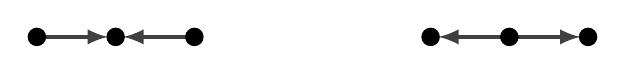
\begin{tikzpicture}
    \SetVertexStyle[FillColor=black, MinSize=0.7]
    \Vertex[x=0, y=0]{n1}
    \Vertex[x=1, y=0]{n2}
    \Vertex[x=2, y=0]{n3}
    
    \Edge[Direct](n1)(n2)
    \Edge[Direct](n3)(n2)

    \Vertex[x=5, y=0]{n4}
    \Vertex[x=6, y=0]{n5}
    \Vertex[x=7, y=0]{n6}
    
    \Edge[Direct](n5)(n4)
    \Edge[Direct](n5)(n6)
    \end{tikzpicture}
\end{center}

Sea $C_{j}$ con $j\geq 3$, el ciclo de $j$ vértices sin cuerdas. Analizar para cada $j\geq 3$ la pertenencia de $C_j$ a la clase de grafos de comparabilidad. Justificar las respuestas (los que son de comparabilidad mostrar la orientación de las aristas, los que no, demostrar que ninguna orientación sirve).
\end{quest}

%%% TERMINA EL EJERCICIO 4 %%%

%%% EMPIEZA EL EJERCICIO 5 %%%

\begin{quest} \verb|[2.5 pts.]|
Labyrinthroid es un videojuego en el cual, en cada nivel, se debe llegar a la meta atravesando un laberinto y derrotando enemigos inmóviles. Tanto el mapa del nivel como la posición de los enemigos son conocidos. 
Se puede considerar como ejemplo el siguiente nivel:

\begin{center}
\begin{tikzpicture}
    \fill[black!40!white] (3,2) rectangle (4,3);
    \fill[black!40!white] (3,0) rectangle (4,1);
    \fill[black!40!white] (1,0) rectangle (2,2);
    \draw[step=1cm,black,very thin] (0,0) grid (4,3);
    \node[inner sep=0pt] (protag) at (0.5, 0.5) {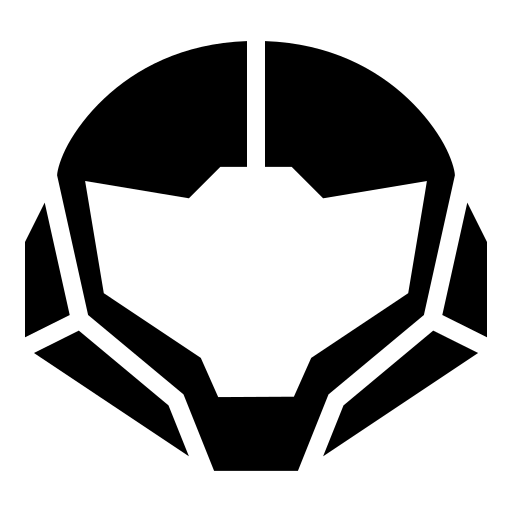
\includegraphics[scale=0.05]{imagenes/protag.png}};
    \node[inner sep=0pt] (monster) at (2.5, 2.5) {
\includegraphics[scale=0.022]{imagenes/monster.png}};
    \node[inner sep=0pt] (door) at (3.5, 1.5) {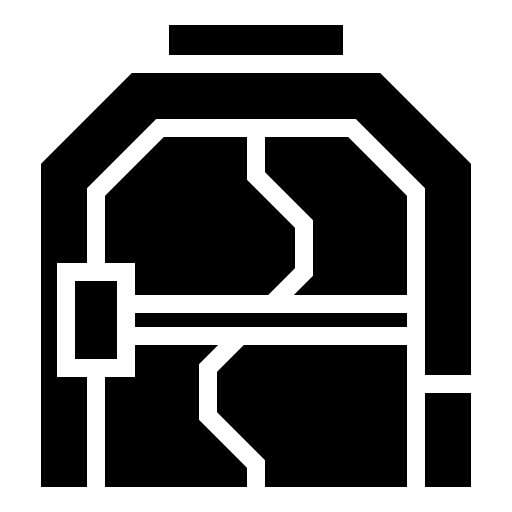
\includegraphics[scale=0.05]{imagenes/airtight-hatch (1).png}};
    \node[inner sep=0pt] (arrow2) at (4.5, 1.5) {
\includegraphics[scale=0.025]{imagenes/arrow.png}};
    \node[inner sep=0pt] (arrow) at (-0.5, 0.5) {
\includegraphics[scale=0.025]{imagenes/arrow.png}};
\end{tikzpicture}
\end{center}

Las reglas son las siguientes:
\begin{itemize}
    \item La protagonista puede moverse a un casillero adyacente en las direcciones $\uparrow, \rightarrow, \downarrow$ o  $\leftarrow $, siempre y cuando no haya un obstáculo (casillero gris). Cada movimiento consume $1$ unidad de tiempo.
    \item Moverse a/desde un casillero donde se encuentra un enemigo consume $2$ unidades de tiempo.
    \item La protagonista tiene la habilidad especial de transformar un obstáculo en un casillero común, pero puede utilizar esta habilidad a lo sumo una vez por nivel. Usar la habilidad no consume tiempo, pero desplazarse a/desde el nuevo casillero habilitado sí.
\end{itemize}
Uno de los logros de Labyrinthroid es finalizar el juego en el menor tiempo posible. Dado un nivel, modelar el problema de llegar a la meta en el menor tiempo posible como un problema en un grafo y proponer un algoritmo que utilice dicho grafo para resolverlo en tiempo polinomial.
\end{quest}

%%% TERMINA EL EJERCICIO 4 %%%

%%% TERMINA EL PARCIAL %%%



\end{document}

